\documentclass[12pt]{article}

\usepackage[french]{babel}
\usepackage[utf8]{inputenc}
\usepackage[T1]{fontenc}
\usepackage{graphicx}
\usepackage{fancyhdr}\usepackage{lastpage}
\usepackage{float}
\usepackage[colorlinks=true,breaklinks=true,linkcolor=blue]{hyperref}
\usepackage{a4wide}
\usepackage[onehalfspacing]{setspace}
\usepackage[left=2cm,right=2cm,top=2cm,bottom=2cm]{geometry}
\frenchbsetup{StandardLists=true}
\usepackage{enumitem}
\usepackage{amssymb}
\usepackage{svg}
\usepackage{algorithm}
\usepackage{algorithmic}
\usepackage{textcomp}
\usepackage{pdfpages}

\pagestyle{fancy}

\setlength{\fboxrule}{0.3mm}
\setlength{\fboxsep}{0.5cm}

\setcounter{secnumdepth}{3}
\setcounter{tocdepth}{2} 

\usepackage{siunitx}

%%%%%%%%%%%%%%%%%%%%%%%%%%%%%%%%%%%%%%%%%%%%%
%%%%%%%%%%%%%%%%%%%%%%%%%%%%%%%%%%%%%%%%%%%%%
%%%%%%%%%%%%%%%%%%%%%%%%%%%%%%%%%%%%%%%%%%%%%

\begin{document}

\thispagestyle{empty}
\begin{center}
\textbf{UNIVERSITÉ D'ANGERS}\\
\textbf{UFR DES SCIENCES}\\
\textbf{DÉPARTEMENT D'INFORMATIQUE}
\end{center}

\begin{figure}[H]
\begin{center}

\includegraphics[scale=0.23]{img/angers.png}
\end{center}
\end{figure}

\begin{center}
\Large{\textbf{RAPPORT}}\\
\Large{\textbf{UE - Algorithme intelligent pour l'aide à la décision}}\\


\textbf{------------------------------------------------------} \\
Algorithme génétique appliqué au problème OneMax  \\
Apprentissage par renforcement pour la sélection intelligente des opérateurs de mutation
\textbf{------------------------------------------------------} \\

\begin{table}[H]
\begin{tabular}{lll}
%\hline
&&\\
%\hline

\end{tabular}

\end{table}

Réalisé par :\\
\textbf{AKMOUCHE Chafik} \\

\textbf{Master 2 Intelligence Décisionnelle} \\
\end{center}

\begin{table}[H]
\begin{tabular}{lll}
%\hline
&&\\
%\hline

\end{tabular}

\end{table}

\begin{center}
2021/2022
\end{center}

%%%%%%%%%%%%%%%%%%%%%%%%%%%%%%%%%%%%%%%%%%%%%
%%%%%%%%%%%%%%%%%%%%%%%%%%%%%%%%%%%%%%%%%%%%%
%%%%%%%%%%%%%%%%%%%%%%%%%%%%%%%%%%%%%%%%%%%%%

\newpage
\renewcommand\headrulewidth{1 pt}\fancyhead[L]{}\fancyhead[C]{}\fancyhead[R]{\textit{Table des Matières}} 
%\addcontentsline{toc}{chapter}{Table des Matières}
\thispagestyle{empty}
\tableofcontents

\newpage
\renewcommand\headrulewidth{1 pt}\fancyhead[L]{}\fancyhead[C]{}\fancyhead[R]{\textit{Algorithmes intelligents pour l'aide à la décision}} 
\setcounter{page}{1}
\pagenumbering{arabic}

\textbf{Résumé}\\

xxxx

\textbf{Mots clés : } Algorithme évolutionnaire, Algorithme génétique, Problème OneMax, Problème de Bandit, PM, UCB.

\section{Introduction}
En l'absence d'une méthode de résolution exacte pour un problème, plusieurs méthodes de recherche de solutions approchées sont utilisées dont les algorithmes génétiques.\\
 
Dans la première partie de ce papier, nous allons parler brièvement des algorithmes génétiques et de leurs objectifs, ensuite nous allons appliquer cet algorithme à l'un des problèmes les plus connus dans ce domaine, à savoir le problème OneMax. Enfin, nous allons discuter les résultats obtenus en testant les différents opérateurs de mutation, croisement, etc.\\

Le nombre de paramètres liés à cet algorithme est très important (plusieurs opérateurs de mutation, croisement, sélection, remplacement...) et il n'y a pas d'opérateur meilleur que l'autre car efficacité de chaque opérateur dépend de plusieurs paramètres et c'est ce que nous allons voir dans les parties suivantes. Afin de résoudre ce problème et répondre à cette question : quel opérateur utiliser et quand l'utiliser ? Nous allons essayer de mettre en place d'un mécanisme permettant de choisir un opérateur \textit{o} à l'instant \textit{t} afin d'augmenter l'efficacité de l'algorithme génétique.\\

Dans la deuxième partie, nous allons donc discuter le fonctionnement de l'algorithme génétique implémenté dans la première partie, ensuite nous allons proposer des solutions qui permettent de choisir intelligemment l'opérateur à utiliser à un instant \textit{t} de l'exécution de l'algorithme génétique. Enfin, nous allons discuter les nouveaux résultats obtenus et faire une comparaison avec les résultats obtenus dans la première partie.

%%%%%%%%%%%%%%%%%%%%%%%%%%%%%%%%%%%%%%%%%%%%%%%%%%%%%%%%%%%%%%%%%%%%%%%%%%%%%%%%%%%%%%
%%%%%%%%%%%%%%%%%%%%%%%%%%%%%%%%%%%%% PARTIE I %%%%%%%%%%%%%%%%%%%%%%%%%%%%%%%%%%%%%%%
%%%%%%%%%%%%%%%%%%%%%%%%%%%%%%%%%%%%%%%%%%%%%%%%%%%%%%%%%%%%%%%%%%%%%%%%%%%%%%%%%%%%%%

\subsection{Rappels sur les algorithmes génétiques}
\par Les algorithmes génétiques appartiennent à la famille des algorithmes évolutionnistes. Leur but est d'obtenir une solution approchée à un problème d'optimisation, lorsqu'il n'existe pas de méthode de résolution exacte.
\begin{itemize}[label=-]
\item Les algorithmes génétiques se basent au départ sur une population de solutions candidates qui va évoluer de génération en génération jusqu’à la génération qui contient les meilleures solutions.
\item Chaque individu comprend des propriétés et il peut être sujet à des transformations génétiques (mutation, croisement...).
\item Chaque individu est évalué et cette valeur d’aptitude (fitness) est un critère pour sa survie d’une génération à une autre.
\end{itemize}

\begin{figure}[H]
		\begin{center}
			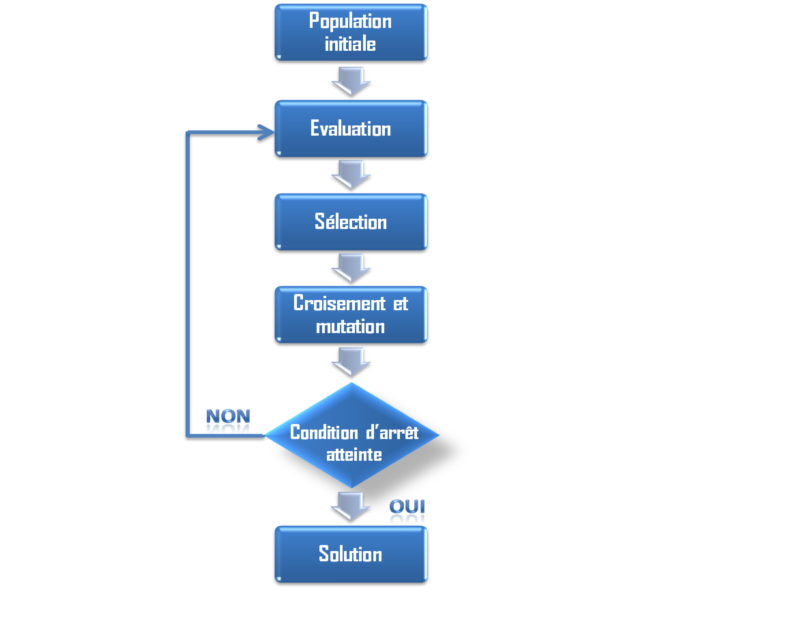
\includegraphics[scale=0.4]{img/algo_genetique.png}
			\caption{Cycle de vie d'un algorithme génétique}
			\label{algo_genetique}
		\end{center}
\end{figure}

\subsection{Rappels sur le problème OneMax}
\par Le problème OneMax est un problème simple qui consiste à maximiser le nombre de uns d'une séquence de bits.
\par Formellement, le problème OneMax peut être décrit comme la recherche d'une séquence (ou un vecteur) $ \vec{x} = (x_1, x_2, ... , x_n) $, avec $ x_i \in \{0,1\} $, qui maximise l'équation suivante : $ F(\vec{x}) = \sum_{i=1}^{n} x_i $

\section{Application de l'algorithme génétique au problème OneMax}
\begin{itemize}[label=-]
\item Une population dans le cadre du problème OneMax est un ensemble fini d'individus;
\item Chaque individu est constitué de gênes (une séquence d'une taille finie de bits 0 ou 1);
\item La population initiale est l'ensemble d'individus initiaux/première génération (n'ayant pas encore subit d'opérations de reproduction);
\item La fitness d'un individu est la somme des bits ayant la valeur 1;
\item La fitness d'une population est la somme des fitness des individus qui la composent.
\end{itemize}

\par À partir de la population initiale, l'algorithme génétique sélectionne un ou plusieurs individus et applique des opérations de reproduction (mutation, croisement...) sur ces derniers, ce qui va générer de nouveaux enfants qui vont remplacer d'autres individus existants dans l'objectif de maximiser la fitness. L'algorithme tourne en boucle jusqu'à ce qu'une condition soit atteinte. 

\section{Implémentation de l'algorithme génétique}
\begin{description}

\item{Paramètres de l'algorithme :} Taille de la population, taille des individus, nombre max de générations, nombre d'exécutions.

\item{Population initiale :} Ensemble d'individus dont tous les gênes sont initialisés à 0.

\item{Sélection :} Représente le choix des individus les mieux adaptés pour les différentes opérations d'évolution.
\item{Opérateurs de sélection implémentés :}  Sélection d'un individu au hasard, 2 individus au hasard, meilleur individu, 2 meilleurs individus et les 2 meilleurs individus sur 5.

\item{Mutation :} La mutation consiste à altérer un gène selon un facteur de mutation (probabilité). La mutation k-flip consiste à altérer k gênes d'un individu selon une probabilité de mutation.
\item{Opérateurs de mutation implémentés : } Mutation 1 flip, bit flip, 3 flip et 5 flip.

\item{Croisement :} Consiste à mélanger les gênes des individus choisis afin de reproduire leurs particularités.
\item{Opérateurs de croisement implémentés :}
\begin{itemize}[label=-]
\item Croisement uniforme : L'enfant issu de ce croisement prend des gênes des 2 parents.
\item Croisement simple : Selon une probabilité, l'enfant prend les gênes du parent 1 ou du parent 2.
\item Croisement mono-point : Création de 2 nouveaux enfants à partir de 2 parents sélectionnés, tel que chaque enfant prend une partie des gênes du parent 1 et l'autre partie du parent 2.

\begin{figure}[H]
		\begin{center}
			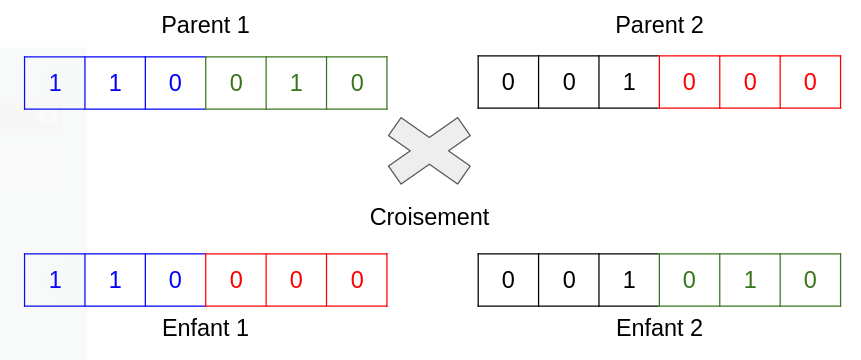
\includegraphics[scale=0.4]{img/crois_mono_point.png}
			\caption{Croisement mono-point}
			\label{crois_mono-point}
		\end{center}
\end{figure}

\end{itemize} 

\item{Remplacement :} Représente le choix des individus à remplacer par les enfants issus des différentes opérations d'évolution.
\item{Opérateurs implémentés :} Remplacement du plus mauvais individu, des 2 plus mauvais individus et des 2 meilleurs individus

\item{Fitness :} $ F(I) = \sum_{i=1}^{n} x_i $   tel que $ I : $ Individu; $ x : $ gêne

\item{Conditions d'arrêt :} Nombre max de générations atteint, population parfaite atteinte (tous les gênes de tous les individus sont à 1).

\end{description}


\section{Fonctionnement général}
La figure \ref{fonct_algo} illustre le fonctionnement général de l'algorithme génétique implémenté ainsi que les différents opérateurs mis en place.

\begin{figure}[H]
		\begin{center}
			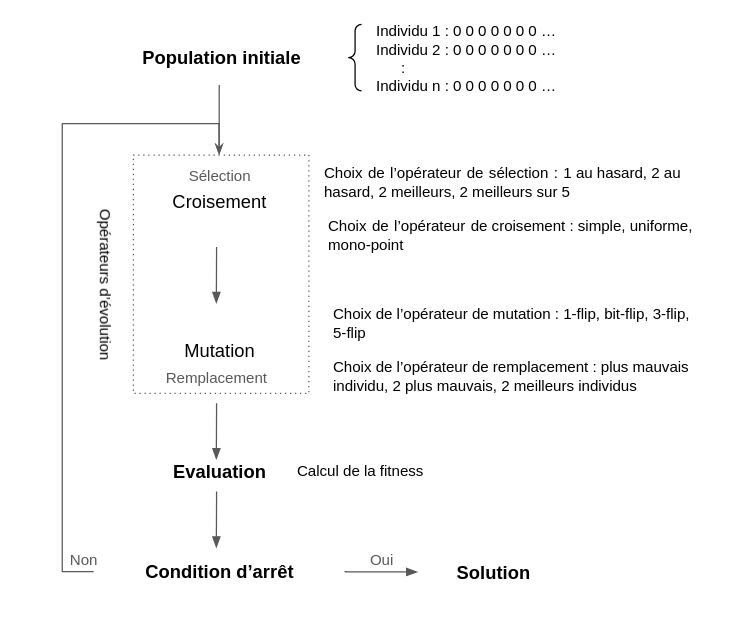
\includegraphics[scale=0.7]{img/fonct-algo.png}
			\caption{Fonctionnement général de l'algorithme génétique implémenté}
			\label{fonct_algo}
		\end{center}
\end{figure}

\section{Résultats}
Vu le nombre important de paramètres de l'algorithme (sélection, mutation, croisement, remplacement), nous ne pouvons pas étudier tous les résultats obtenus des différents paramètres. Dans cette étude, nous allons nous focaliser beaucoup plus sur les résultats liés à la mutation.
\begin{enumerate}
\item{Résultats en fonction des opérateurs de mutation :} La figure \ref{fitness_op_select} montre l'évolution de la Fitness max obtenue sur 20 exécutions différentes en fonction des opérateurs de mutation (1-flip, bit-flip...).
\begin{itemize}
\item{Paramètres de l'algorithme :}
	\begin{itemize}[label=-]
		\item{Taille de la population : } 400
		\item{Taille de l'individu :} 1000
		\item{Max génération :} 400
		\item{Nombre d'exécution :} 10
		\item{Opérateur de sélection :} Sélection des 2 meilleurs individus de la population.
		\item{Opérateur de croisement :} Croisement mono-point.
		\item{Opérateur de remplacement :} Remplacement des 2 plus mauvais individus de la population.
		\label{param_algo_1}
	\end{itemize} 

\begin{figure}[H]
		\begin{center}
			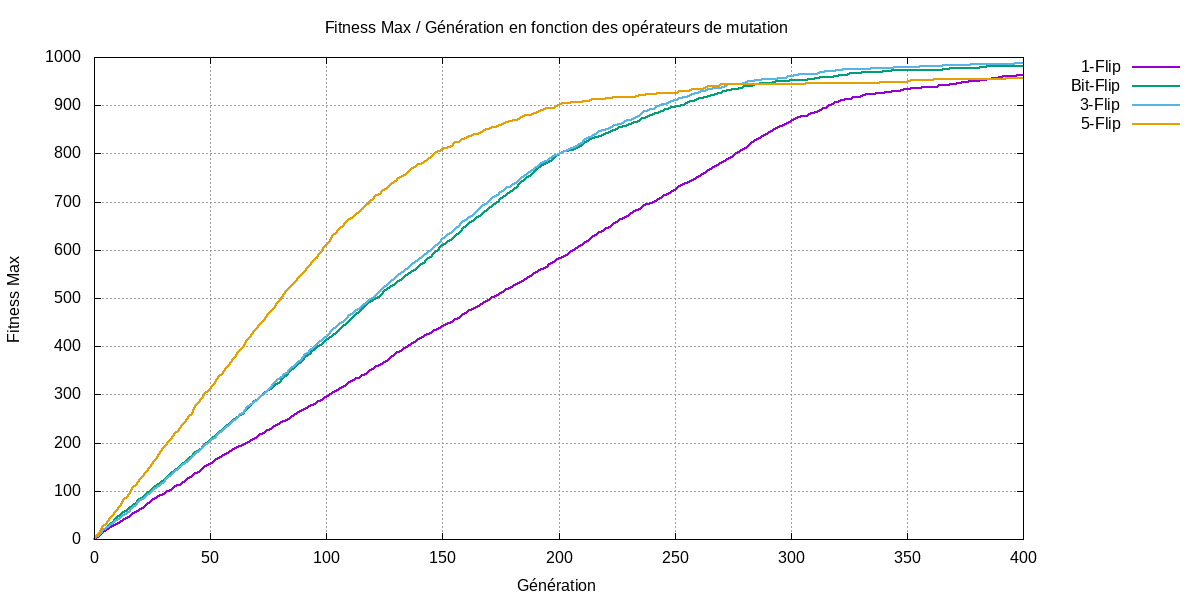
\includegraphics[scale=0.5]{img/fitness_op_select.png}
			\caption{Évolution de la Fitness Max en fonction des opérateurs de mutation}
			\label{fitness_op_select}
		\end{center}
\end{figure}

\item{Discussion :}

\end{itemize}
%\begin{table}[H]
%\begin{center}
%\begin{tabular}{|c|c|c|c|c|}
%\hline  
%- & \multicolumn{4}{c|}{Fitness moyenne sur 20 exécution}  \\
%\hline
%Génération & 1 Flip & Bit-Flip & 3 Flip & 5 Flip \\
%\hline
%1 & 0 & 0 & 0 & 0 \\
%\hline
%\end{tabular}
%\end{center}
%\end{table}
\item{Résultats en fonction des opérateurs du croisement : } La figure \ref{fitness_op_crois} montre l'évolution de la Fitness max obtenue sur 20 exécutions différentes en fonction des opérateurs du croisement (croisement simple, uniforme et mono-point).
\begin{itemize}
\item{Paramètres de l'algorithme : }  Nous avons utilisé les mêmes paramètres que (\ref{param_algo_1}). 
	\begin{itemize}
	Opérateur de mutation : Mutation Bit-Flip.
	\end{itemize}  
 
\begin{figure}[H]
		\begin{center}
			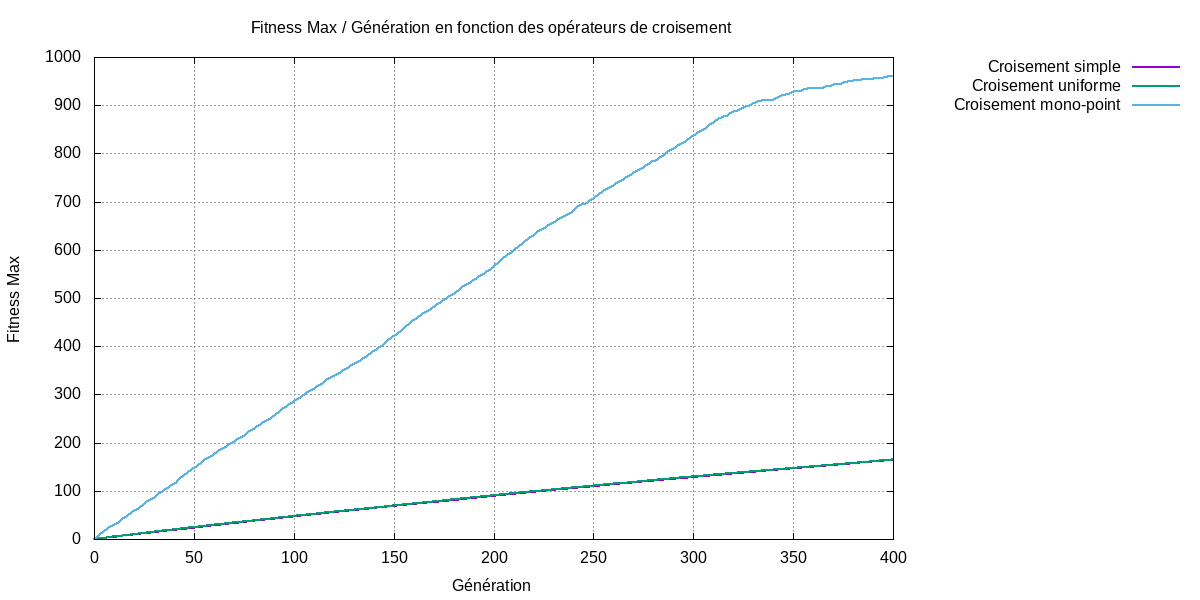
\includegraphics[scale=0.5]{img/fitness_op_crois.png}
			\caption{Évolution de la Fitness Max en fonction des opérateurs du croisement}
			\label{fitness_op_crois}
		\end{center}
\end{figure} 

\item{Discussion :}
\end{itemize}

\end{enumerate}

%%%%%%%%%%%%%%%%%%%%%%%%%%%%%%%%%%%%%%%%%%%%%%%%%%%%%%%%%%%%%%%%%%%%%%%%%%%%%%%%%%%%%%
%%%%%%%%%%%%%%%%%%%%%%%%%%%%%%%%%%%%% PARTIE II %%%%%%%%%%%%%%%%%%%%%%%%%%%%%%%%%%%%%%
%%%%%%%%%%%%%%%%%%%%%%%%%%%%%%%%%%%%%%%%%%%%%%%%%%%%%%%%%%%%%%%%%%%%%%%%%%%%%%%%%%%%%%

\section{Problématique du choix du meilleur opérateur}
Le choix de l'opérateur à utiliser comme nous l'avons vu dans la section précédente affecte d'une manière directe la Fitness ou l'efficacité de l'algorithme génétique d'une manière générale.\\

Dans cette étude, nous allons nous intéresser aux opérateurs de mutation. Nous avons vu dans la partie précédente que l'efficacité des opérateurs dépende directement de la taille du problème et de l'instant lorsque l'opérateur est utilisé. Nous avons vu qu'au début de l'exécution (0 - 200 génération) l'opérateur 5 Flip était plus améliorant que les autres opérateurs, mais à partir de la génération 200 nous avons remarqué l'inverse.\\

Une amélioration qui peut augmenter considérablement la Fitness serait donc de mettre en place un mécanisme qui permet de choisir intelligemment à un instant \textit{t} l'opérateur \textit{o} à utiliser.\\

Il existe plusieurs méthodes qui permettent à partir d'un certain nombre de données en entrée de décider de quelle action effectuer à un instant \textit{t} afin de maximiser le gain.

\paragraph{Définition du problème :} Nous avons :
\begin{itemize}[label=-]
\item 4 opérateurs de mutation : 1 Flip, Bit-Flip, 3 Flip, 5 Flip. 
\item Un nombre max de générations.
\item Une fonction Fitness (fitness cumulée qu'on cherche à maximiser).
\end{itemize}
\paragraph{Objectif : } À chaque itération (génération), l'algorithme doit pouvoir choisir le meilleur opérateur de mutation qui permet de maximiser la fitness cumulée. 

\section{Algorithme du Bandit}
\paragraph{Problème du bandit : } Afin de simplifier le problème du bandit, nous allons prendre le cas le plus simple. On considère une machines à sous à 2 bras, notés A et B. L’action du bras A (resp. B) donne lieu à un gain qui n'est pas connu a priori, et le joueur cherche à actionner le bras le plus favorable. L'idée consiste à choisir un bras au hasard, mais en modifiant au cours du temps la loi de probabilité du choix du bras, i.e. Si à l’étape $ n $, le bras actionné avait une probabilité $ p_n $ d’être choisi, s’il produit un gain, on lui affecte à l’étape suivante une probabilité plus importante $ p_{n+1} \ge p_n $.

\paragraph{Algorithme de bandit : } L'algorithme du bandit tient son nom du problème expliqué dans le paragraphe précédent où le joueur cherche à maximiser son gain. L'algorithme du bandit est un modèle d'apprentissage par renforcement qui consiste à un instant $ t $ de choisir l'action $ a $ dont il a appris qu'elle récompense beaucoup.\\

\par Dans notre cas, les k-bras de la machine à sous (multi-armed bandit) sont les différents opérateurs de mutation et à chaque génération l'algorithme choisit un opérateur et ajuste les probabilités du choix des opérateurs en fonction des gains.

\paragraph{Récompense : } La récompense est la valorisation immédiate d’une action dans un état donné : $ R_t = Fitness_t - Fitness_{t-1} + d $ \\tel que $ d $ est la valeur de décalage qui permet de ne pas avoir une récompense négative.\\

\par Il existe plusieurs approches (politiques) pour résoudre ce problème : $ \varepsilon- $Greedy, Probability Matching, Upper-Confidence Bound (UCB), Lower Upper Confidence Bound (LUCB), etc.\\

\par Dans notre cas, nous avons implémenté les deux algorithmes "Sélection par roulette proportionnelle" et "UCB".


	\subsection{Sélection par roulette proportionnelle}
	Au lancement de l'algorithme, tous les opérateurs ont une probabilité $ P_{init} = \frac{1}{nb\_operateurs} $. Dans notre cas, nous avons 4 opérateurs, donc la probabilité initiale de chaque opérateur $ P_{init} = \frac{1}{4} $. L'algorithme choisit donc aléatoirement un opérateur, calcule l'amélioration/récompense immédiate et le gain pour ajuster les probabilités des opérateurs.\\
	$ \pi_i^{t+1} = P_{min} + (1 - N.P_{min} ) \frac{u_i^{(t+1)}}{\sum_{k=1}^N u_k^{(t+1)}} $\\
	Tel que : \\
	
		\subsubsection{Application}
	\subsection{UCB}
		\subsubsection{Application}

\section{Analyse et discussion des résultats obtenus}

\section{Conclusion}

\end{document}